
\begin{answer}
I used GPT-5.4 for E, F, and Z in place of the original Gemini setup.
E was instructed to answer verbosely; F had no length instruction. For each
of the 30 AlpacaEval questions, Z saw the question and both answers under
anonymous labels A and B, with E appearing first in 15 pairs. The judge
prompt prioritized accuracy, relevance, and useful details and explicitly
told Z not to reward length by itself. It asked for a short rationale and
a final line in the format \texttt{WINNER: A} or \texttt{WINNER: B}.
The script extracted the last line and mapped the anonymous winner back
to E or F. The original responses, judge rationales, and labels are saved
in \texttt{alpaca\_judgments.json}.

\input q_llm_judge_stats

\begin{center}
    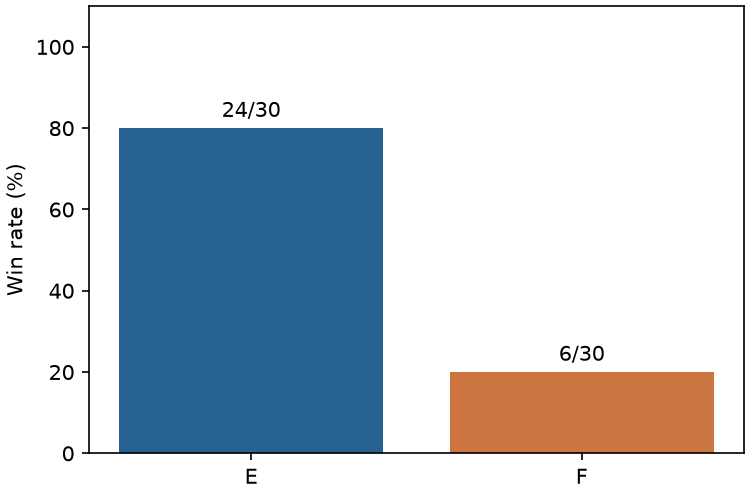
\includegraphics[width=0.55\linewidth]{static/alpaca_win_rates_gpt54.png}
\end{center}
\end{answer}
